\chapter{CRM enhanced by Artificial Intelligence}
\label{sec:crm-ai}


% -------------------------------- Section: What is a CRM
\section{Customer Relationship Management}

% What is a CRM
With a total market revenue of \$39.5 billion in 2017 and an expected growth rate of 16\% for 2018, Customer Relationship Management (CRM) is the largest segment of enterprise applications \cite{gartner-crm-market}. From its most basic form as an \textit{Excel} spreadsheet to \textit{Software-as-as-Service} (SaaS) solutions, a CRM is an approach for managing an organization's relationship and interactions with current and potential customers alongside with the data and information associated to them \cite{salesforce:CRM-def}.

% Why is it useful
There are many possible descriptions for customer relationship management. At high-level, it as a transversal organizational strategy that allows a company to better understand, anticipate, and manage the needs of current and potential customers. The whole philosophy of a CRM is to place the customer at the heart of the system \cite{brown2000customer}\nocite{biedermann-crm}. A CRM has tools to follow, understand, and nurture all interactions between a company and its customers. It supports the relationship through the entire customer life-cycle, from the prospects to loyal customers. 

CRM systems aim to maintain a good relationship with customers, which leads to a better service and revenues for the company. Indeed, studies have pointed out that managing long-term relationships with clients is worth the effort, because it's five times more expensive to acquire new customers than retaining current ones \cite{crm-facts}. Developing and focusing solely on products is not an option for companies because bad user experience will hurt the business in the long-term\footnote{It's reported that one unsatisfied customer talks to 12 other customers while one satisfied customer talks to four others. Businesses must be willing to sacrifice short term advantage for long term gains \cite{crm-facts,bennet,crm-essay}}.

% What a CRM does
An important aspect of CRM systems is its ability to store and share data. From the first contact with a customer until the last question asked to the customer service, all customer-related data is saved and shared across company's departments. It avoids data silos and incomplete information within the same enterprise. Also, it enables to have a 360° vision of the customer relationship with all touchpoints inside the company \cite{efficy-crm}.

A CRM can also be viewed as a set of macro-level process that subsumes numerous sub-processes \cite{crm-processes}. These processes must be aligned between the business's needs and IT operations. As shown in figure \ref{fig:crm-clc}, these functional processes support the entire customer life cycle.

\begin{figure}[h]
    \centering
    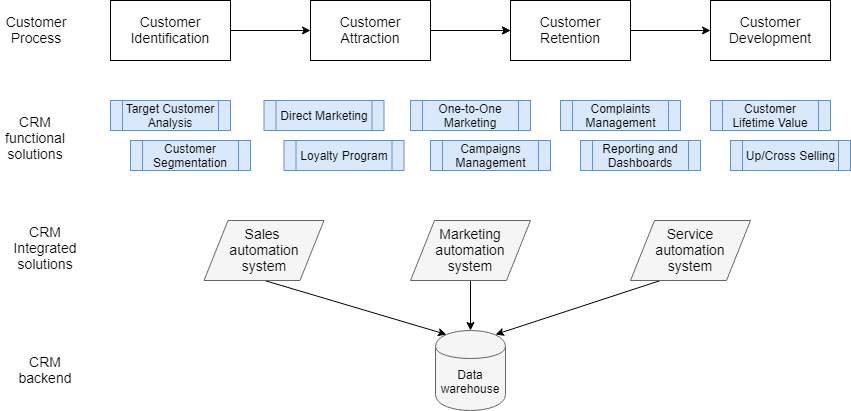
\includegraphics[width=12cm]{images/CRM-CustomerLifeCycle.png}
    \caption[CRM supports the customer life cycle]{CRM supports the customer life cycle. From \cite{DataAnalyticsinCRMProcessesALiteratureReview}.}
    \label{fig:crm-clc}
\end{figure}

% How it does it
CRM systems are usually organized around four axes: Sales, Marketing, Support and Analysis \cite{crm-def}. The first three belong to the operational part of a CRM, used for lead generation and conversion for example. The analytical part of the CRM analyzes and generates insights from the data collected by the operational processes. Through the years, CRM systems produce and store more and more data. \textit{Big data} techniques are employed to make use of them, instead of just having them stored \cite{peel-et-al}.


% -------------------------------- Section: Why AI within CRM
\section{CRM AI}

CRM AI is a term often found in blogs, forums and other CRM literature. But what does it really means? Is it more than just a buzzword? Are CRM systems made intelligent with AI? This section details the motivations for combining CRM+AI and the questions and interrogations arising from.

\subsection{Artificial Intelligence within CRM}

Often cited as the next major vague of innovaiton, Artificial Intelligence (AI) can be the tool to optimize customer interactions based on the amount of data companies have. In its \textit{IT Glossary}, Gartner defines AI as a technology that appears to emulate human performance \cite{gartner-glossary}. AI learns, comes to its own conclusion, appears to understand complex content, can engage into a natural conversation with people, enhances human cognitive performance or replaces people in the execution of nonroutine tasks.

In a customer relationship management context, artificial intelligence can be used to enhance the functionalities of a CRM. AI relies on data and all the customer-related data that a company has is stored in its CRM. By applying AI technologies into CRM applications like sales or service automation, current processes can evolve and new functionalities to drive user decisions be created. AI has the ability to ingest data and assist CRM's user in their daily tasks, whether by intelligently analyzing a large volume of data or by being proactive and anticipating needs. The aim is to create a more personalized customer experience with the insights uncovered by AI techniques. Once mastered and integrated, these new AI insights will make a business \textit{smarter}.


\subsection{Outline of the analysis}
% -------- Goal of the analysis
One of the aims of this thesis is to provided an overview of the integration of artificial intelligence technologies in a CRM context. With the advent of artificial intelligence and its relative ease of access, CRM vendors can consider a new product line around AI. When a CRM editor announces the integration of AI components in its solutions, it aims to attract new customers while showing current customers that its system is innovative.

CRM editors claim to have easy to use and well integrated AI solutions, but what is offered in these solutions? What are the kind of AI technologies used? How easy to configure are those AI features? Are they really tailored and useful for the business? All companies are different, but can they adapt these innovative solutions to their unique business? What AI functionalities will become \textit{mandatory} for a good CRM? The research in this section tries to address those issues and really understand what is meant by \textit{CRM AI}.


% -------------------------------- Section: Editors Market
\section{Editors Market}


\subsection{CRM Editors analyzed}
The CRM software market is growing rapidly, especially due the awareness of customer experience's importance and the expansion of cloud-based solutions \cite{crm-revenue}. Indeed, all types of companies, regardless of their size or revenues, can have their own CRM without the need to invest in hardware. Opposed to on-premise deployments where the CRM runs in an infrastructure created and maintained by the company, cloud-based deployment are today the most request deployment configuration\footnote{In 2008, only 12\% of the requests for CRM had a preference for cloud-based deployment. Six years later the trend is totally reversed, with 87\% of the deployment's requests regarding cloud-based solutions and 13\% on-premise CRMs \cite{crm-deployment-stats}.}.

There are a lot of offers in the CRM market\footnote{For example, \textit{Wikipedia} lists a total of 29 CRM systems.}. Some editors build complete CRM solutions while others focus on one or two applications, such as sales force automation or customer engagement solutions. The editors analyzed in this project have been selected based on Gartner's \textit{Magic Quadrant}\footnote{Gartner is a research and advisory firm providing analysis on the Information Technology (IT) field.}. Two types of magic quadrant are directly related to customer relationship management: sales force automation and customer engagement (figures \ref{fig:magic-quadrant-sales-force} and \ref{fig:magic-quadrant-customer-engagement}). A magic quadrant contains four groups and all global CRMs classified as \textit{Leaders} are considered : \textit{Salesforce}, \textit{Microsoft}, \textit{Oracle} and \textit{Pegasystems}. Despite not being classified as a \textit{leader}, \textit{SAP} is also considered since it is the third largest publisher \cite{crm-market-share}. These five CRMs are the big fishes in the market (40.4\% of the market) and have the stongest R&D departments: they are the most likely to invest in AI features. Nevertheless, to stand out in the market, smaller companies specialize their products around a specific CRM's application. To be as complete as possible, \textit{SugarCRM}, \textit{Infor}, \textit{Zoho} and \textit{Zendesk} are also investigated.

\begin{figure}[!h]
    \begin{minipage}[c]{0.48\linewidth}
        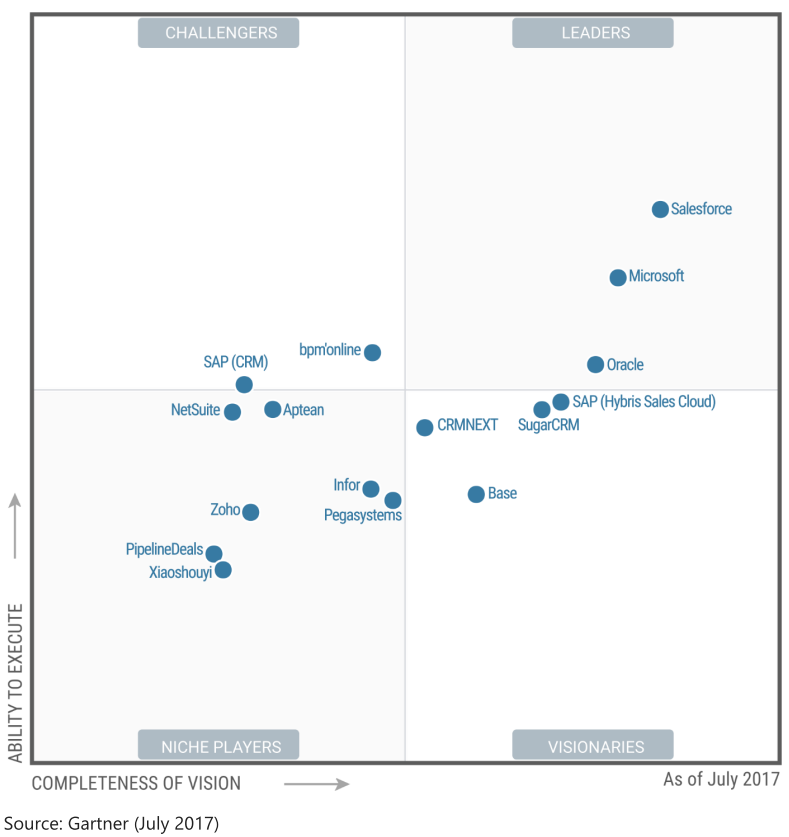
\includegraphics[width=\linewidth]{images/magic_quadrant_sales_force_automation.png}
        \caption[Magic Quadrant for Sales Force Automation]{Gartner, Magic Quadrant for Sales Force Automation, July 2017}
        \label{fig:magic-quadrant-sales-force}
    \end{minipage}
    \hfill
    \begin{minipage}[c]{0.49\linewidth}
        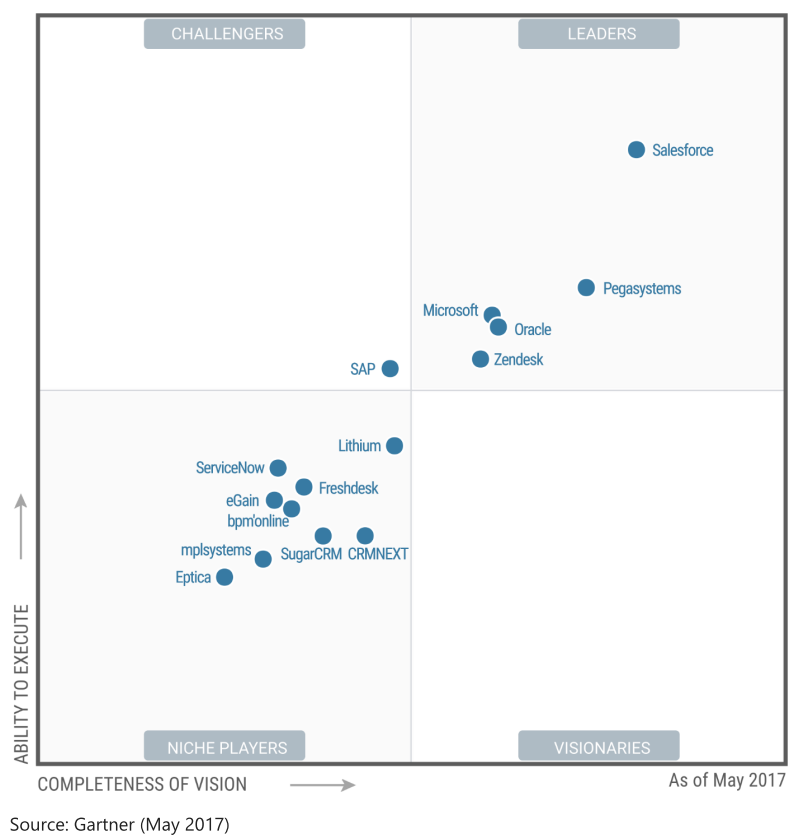
\includegraphics[width=\linewidth]{images/magic_quadrant_customer_engagement_center.png}
        \caption[Magic Quadrant for the CRM Customer Engagement Center]{Gartner, Magic Quadrant for the CRM Customer Engagement Center, May 2017}
        \label{fig:magic-quadrant-customer-engagement}
    \end{minipage}
\end{figure}

To analyze all those CRM solutions, company's website, press releases, community forums and knowledge base articles are used. Blog posts, specialized websites, and analyst firm's report are also widely used. Note that it was not possible to configure and test the functionalities detailed in the following sections. Products and features announced by CRM's editors after April 2018 are not taken into account in this research.

\subsection{CRM Editors review}

\subsubsection*{Dynamics 365}
Dynamics 365 is the customer relationship management solution of Microsoft. Created in 2003 as Microsoft Dynamics CRM, the product was rebranded Dynamics 365 when an Enterprise Resource Planning (ERP) solution has been combined with the CRM. One of the key characteristics of Dynamics 365 is its native integration with other Microsoft products, like Microsoft Exchange, Office 365, Sharepoint and PowerBI. More recently, Dynamics 365 is building synergies with Azure technologies, which seems to be the foundation for AI inside Dynamics 365. 

Mid-2017, Microsoft launched the preview program of \textit{Dynamics Customer Insights}, a combined product of Azure and Dynamics 365. Available through the Azure portal (therefore not built-in the CRM), this product can support an entire machine learning project, from data collection to result's visualization. The data from Dynamics 365 can be combined under a new datamodel with external data stored in \textit{csv} files. If common unique ids aren't available between these datasets, the tool uses Natural Language Processing (NLP) techniques to link the data together, based on a name, a street address or a phone number for example. The user can then select a variable (continuous number or boolean value) and a predictive machine learning model is trained with the data imported into \textit{Dynamics Customer Insights}. The model is probably a linear model generated with \textit{AutoML} techniques\footnote{Automated Machine Learning, abbreviated \textit{AutoML}, are algorithms to automatically select a good model, choose its hyperparameters, and perform features preprocessing steps for a new dataset \cite{NIPS2015_5872}.}. With the model generated, \textit{Dynamics Customer Insights} can use the predictions to create customer segments and visualizations. For example, the risk of churn\footnote{A score between 0 and 100 which indicates how likely a customer is of \textit{leaving} the company.} can be computed based on a predictive model.

AI features directly built-in Dynamics 365 are not yet available for everyone, but Microsoft releases some preview features such as intelligent suggestions and lead scoring. Intelligent suggestions recommends the knowledge based articles best-suited to deal with a customer's question in the CRM's ticket system. Lead scoring assigns a score for each lead (a potential new customer) based on the lead's profile and all previous leads stored in CRM's historical data.

Dynamics 365 hasn't yet any AI feature available for production, but Microsoft has such products in its Azure platform. Dynamics for Customer Insights is one example and the program will be relaunched in Fall 2018. Another Azure product for which existing interactions exists with Dynamics 365 is the Microsoft Bot Framework. This SaaS allows users to create chatbots. NLP models for intent and entity recognition are trained from a visual interface and the bot can interact with Dynamics 365 via its Web API.

\subsubsection*{Infor CRM}
Infor is a business cloud application provider that offers a CRM as part of its \textit{Customer Experience Suite}. Named Infor CRM, the product is composed of sales, marketing, and customer service applications. In July 2017, Infor announced \textit{Coleman}, an AI platform available as a virtual assistant. Accessible by voice or chat, CRM users use it to perform simple and predefined tasks, such as searching contact informations or aggregating sales revenue for the last month. Infor CRM is available as a \textit{SaaS} hosted in \textit{Amazon Web Services} (AWS) and Coleman was built with \textit{Amazon Lex}, a product to build conversational interfaces. This seems to be Infor's strategy for AI: using existing frameworks such as AWS to extend their CRM functionalities.

Infor also claims to have a sales intelligence for CRM, with features that give insights about the next likely purchase of a customer, the customer's risk of churn and client segmentation based on their purchase history. It is not clear if those features are already implemented, as they only appear in Infor's marketing content.\nocite{infor-website}


\subsubsection*{Oracle}
Second-largest software maker by revenue after Microsoft, Oracle proposes CRM solutions via two products: \textit{Oracle Siebel} for on-premise deployments and \textit{Oracle CRM} for SaaS. Only available for the cloud, \textit{Adaptive Intelligence} applications have been announced in 2017. Instead of regrouping all their AI solutions under a general brand name, Oracle claims to \textit{avoid the hype and focusing on building apps that people can make money with }\cite{crm-techmerge}. The philosophy is to build ready-to-use applications that CRM users can quickly integrate into their current system and add a layer of \textit{intelligence}.

These adaptive intelligent applications\footnote{\textit{Adaptive Intelligent} apps can also be abbreviated \textit{AI} apps...} concern several areas of customer relationship management, from the sales (next best sales actions or lead scoring) to the customer service (automated answers) to the marketing division (audiences segmentation, optimized campaign channel, and optimized contact time). Despite having been in contact with Oracle's team, it was not possible to have a list of the applications already available or to have details about some features, like the \textit{next best sales actions} feature. It seems that artificial intelligence components to be integrated into Oracle CRM are at an early stage of development and not ready to be used by users. 


\subsubsection*{Pega CRM}
Pegasystems Inc. is a software company developing a CRM product based on the company's expertise with business process management (BPM). Pega CRM's revenue is highly dependent on its on-premise solution: \textit{SaaS} is estimated to represent only 8\% of the total revenue according to Gartner. This explains why Pegasystems is the only CRM's editor in this study to propose AI features for both on-premise and cloud deployments.

Artificial Intelligence solutions are divided into two products. There is a virtual assistant with a chat and pre-built integration for Facebook Messenger and Amazon Alexa. This assistant has no functionalities or scenarios: it is meant as a development framework with out-of-the-box NLP and text analytics capabilities, such as intent and entity detection. CRM developers can built their own scenarios and processes. The virtual assistant can also be integrated to handle incoming emails. Such \textit{email assistant} can analyze the content of an email and redirect it to the most appropriate person.

A second product available in Pega CRM is named \textit{Customer Decision Hub}, a centralized set of AI capabilities deployed across CRM applications. For the marketing, a recommender system is used to propose the most appropriate product to customers. The sales application contains a lead and opportunity scoring feature as well as a customer's risk of churn evaluation. There are also two products that have been announced recently. First, an AI-coach for salespeople providing personalized advices and tips to under-performing sellers. Then, an update on the \textit{Customer Decision Hub} will enable users to build machine learning models and integrated them directly into CRM's processes. This tool is meant to build predictive models in a similar way as \textit{Dynamics Customer Insights} does, but the user can choose the type of machine learning model to use. Models are saved in the \textit{Predictive Model Markup Language} (PMML) language\footnote{PMML is an XML file format for predictive models that can be exchanged between different analytical applications. It can contain data transformations (pre- and post-processing) as well as one or more predictive models \cite{pmml}.}. This enables users to import their own models, but with some restrictions on the type of models imported. Models can also be defined as an \textit{Adaptive analytics} model that will be retrained when new customer data is available.

\subsubsection*{Salesforce}
Created in 1999 and providing only cloud solutions, Salesforce is the worldwide leader regarding customer relationship management systems. Between 2015 and 2016, Salesforce acquired several AI start-ups and build a team of 150 data engineers. This strategy enabled the company to launch Salesforce Einstein, an artificial intelligence solution spanning over all CRM's products.

For a company's sales department, Einstein offers lead scoring to prioritize client's the most likely to convert and a forecasting feature to estimate the sales for each salesperson. It also gives client's \textit{insights} such as its overall happiness score. This score is computed with sentiment analysis on emails but also company-specific information based on the news (for example if its share price falls on the stock market, the client will be unhappy). Marketing's departments can use Einstein for it mass mailing operation and bring some personalization into the emails. For example, based on recommender systems, the email can integrate a link to a specific product that customers are successive to buy. The \textit{Email Engagement Prediction} feature predicts for each customer its likelihood to open an email or unsubscribe from the newsletters. These predictions can be used to send different contents for each customer and personalize the message. For the customer service's department, Salesforce can classify incoming customer tickets with Einstein and has announced recommended responses and intelligent routing for mid-2018.

All features mentioned above are configurable without any coding-skills, but Salesforce created \textit{MyEinstein}, an API-based service to build custom applications. As of March 2018, this tool was composed of the beta versions of \textit{Einstein Bots} with entity, intent, and sentiment analysis and of \textit{Einstein Prediction Builder} to build predictive models, similar to Dynamics Customer Insights.

Salesforce has two major partnerships regarding AI: one is with \textit{Google Analytics} to create better customer segmentation and another one with \textit{IBM Watson} to improve Einstein's abilities regarding unstructured data and problem-solving tasks.

\subsubsection*{SAP}
The SAP company, short for \textit{Systeme, Anwendugne und Produkte in der Datenverarbeitung}, sells enterprise software such as an ERP or a CRM. SAP has two products for customer relationship management: SAP CRM 7.0 for on-premise configurations and SAP Hybris Service Cloud for online deployments. Only the last one benefits from \textit{SAP Leonardo}, the platform used by SAP to integrate AI features across all their cloud products. The company claims that SAP Leonardo can be used for analytics, machine learning, big data, blockchain, and Internet of Things (IoT).

Regarding SAP Hybris, several products relying on AI have been announced, such as \textit{SAP Hybris Customer Attribution} to segment customers based on game theory, \textit{SAP Resume Matching} to classify candidatures and speed up the recruitment process, \textit{SAP Cash Application} to match payments received with open bills, and \textit{SAP Service Ticket Intelligence} to route customer service tickets to the appropriate agent, assign a priority score to each ticket and proposed knowledge base articles to resolve it. These solutions are meant to be available from the CRM without any coding-skills required to set them up. SAP also plans to offer \textit{SAP Leonardo Machine Learning} to create machine learning algorithms based on TensorFlow models, but there's no information about how these models are built\footnote{TensorFlow is a library used for machine learning applications an in particular neural networks projects.}. This product as some pre-built services such as image recognition (object classification, face recognition) and text analytics (topic detection, similarity scoring). 

SAP is investing a lot in the AI for business field with two products announced for mid-2018: \textit{SAP Leonardo Conversation AI Foundation} to build chatbots and \textit{SAP Predictive Analytics} to build predictive machine learning models in the same manner as \textit{Dynamics for Customer Insights}, but for on-premise solutions.


\subsubsection*{SugarCRM}
SugarCRM is the most important CRM's editor relying on an open-source technology. Back in 2016, SugarCRM announced its plans regarding the usage of AI inside CRM. Two products were under investigation. The first was \textit{Candace}, an AI-powered intelligent agent to assist users in their daily tasks, such as setting up meetings, throwing reminders or monitoring social networks to spot client's dissatisfaction signs. Another announcement concerned the \textit{Sugar Intelligence Service} product to bring AI-features like lead scoring or text sentiment analysis into the CRM. Since then, no evolution has been announced. By analysing blog posts written by SugarCRM's head of corporate strategy, artificial intelligence features are not a priority. SugarCRM is taking a \textit{wait and see} approach \cite{sugarcrm1,sugarcrm2} regarding the subject.

\subsubsection*{Zendesk}
Zendesk is not a global CRM, it has no sales force automation nor developed marketing product. Nevertheless, it is one of the leaders for customer support solutions. Zendesk offers AI functionalities regarding customer's tickets: redirection to the most appropriate person, automated prioritization, and customer risk of churn. It can compute a satisfaction prediction score for each customer, based on the ticket content and client's support history. Zendesk also offers a framework to develop chatbots.

\subsubsection*{ZohoCRM}
Zoho Corporation is specialized in developing business and IT solutions available as SaaS. The CRM - \textit{ZohoCRM} - has all its AI features regrouped under \textit{Zia}, described as an artificial intelligence powered sales assistant. Triggered by voice or chat, the Zia assistant performs some pre-defined tasks such as adding a note to a meeting or retrieving client's contact information. Zoho provides an user-interface to create new capabilities for Zia without any coding- skills required.

Zia is a chatbot but it also encapsulates other AI features of ZohoCRM, among which lead scoring, anomalies detection to control sales, email sentiment analysis and an indication on the best time to contact each client. It also proposes a feature to monitor the tasks performed by CRM's user and proactively suggest new processes for a better efficiency. It's not clear if artificial intelligence techniques are really being used for these functionalities. While it is obvious that email's sentiment analysis relies on NLP algorithms, the anomalies detection or best time to contact a client features can be done without any kind of AI. Those AI features are black-boxes to be used \textit{as-is} in the CRM.


% -------------------------------- Section: Editors Ranking
\section{CRM Editors Ranking}
After analyzing each editor separately, the results are compared to have a general overview of customer relationship management extended with artificial intelligence.

\subsection{Current state}
Among all AI features observed, four of them are expected to become widespread and be integrated into the majority of CRM systems in the next 12-18 months:

\begin{itemize}
    \item \textbf{Lead scoring and risk of churn}: Those two features are based on predictive machine learning models and are already implemented by some CRMs. Results are stored in a new variable, users can be ranked based on it, and any CRM process can easily integrate those results in its execution. The models are trained on historical data: all leads that turned or didn't turn into clients for the lead scoring feature and all clients who've left or not the company for the risk of churn. More generally, predicting activities is a great application of CRM data.
    \item \textbf{Product recommendation}: Recommender systems are well-studied in the machine learning literature and have been applied to real-world data since some years (Amazon and Netflix are two such examples). Not surprisingly, CRM's editors have built such tools. Based on customer's characteristic and purchase history stored in a CRM, product recommendations can bring huge value to the marketing processes and add a layer of personalization when dealing with customers.
    \item \textbf{Customer service tickets}: The customer service applications of a CRM can be extended with AI capabilities, such as assigning a ticket to the most appropriate agent and generate answers with the knowledge base articles. Based on NLP techniques like sentiment analysis and topic modeling, these features can drastically improve the efficiency of the customer service, which is critical for a company's image.
    \item \textbf{Virtual assistants}: Even if they are not exclusive to customer relationship management, chatbots are investigated and integrated by CRM's editors. Chatbots can interact directly with customers and support simple requests, for example recording a new address. It leaves more time for human agents to handle more complex cases. Moreover, if a chatbot doesn't understand or can't solve a customer's request, it can escalate the question to a human. There is also another type of bots: chatbots internal to a company that act as an assistant for CRM's users. There will likely be more and more use cases and scenarios in the future with virtual assistants to extend CRM.
\end{itemize}

The four functionalities above are the most mature ones to be integrated into productive CRM systems. Among all other features, predicting the optimal time to contact a client is very interesting and can be used by all applications of a CRM. Nevertheless, the current solutions don't seem to use AI techniques. Instead, they rely on simple statistics about when a customer has opened its email the more often. An equally promising set of features is related to the marketing application and its mass emailing processes. Salesforce has a feature to predict if a user will open an email or click on a link inside it. This feature can be improved and bring real value if the content of the email is taken into consideration by the model. Marketers will be able to change the content of their emails and reach a larger audience. Another feature for the marketing part of a CRM deals with the customer fatigue. Machine learning models can avoid sending too much marketing content to a given customer and prevent unsubscriptions. Currently, those types of features aren't yet proposed but CRM's user can expected them to be in further releases.

Using AI capabilities inside existing CRM processes is new. To be adopted and used, CRM's users may feel the need to understand why an artificial intelligence algorithm advises this or that action. For example, within its lead scoring component, Salesforce Einstein indicates the main factors that influenced the score. It is probably based on the weights and feature importance of the machine learning model, most likely a linear or tree-based model.

Most of the features described above are directly available as black-boxes. Some can be slightly configured or tuned, but none can be completely customizable. Such deployment is perfect for general features that concern the majority of companies, like the lead scoring component. But in order to have AI features from which a business can fully benefit, they must be tailored for the company's specific needs. Pega CRM is the only one allowing users to import their own custom models. Without going that far, Salesforce and SAP have created REST APIs for pre-trained NLP features such as sentiment analysis, document similarity scoring, and document feature extraction. Users can leverage those models to build custom applications faster. Dynamics 365 doesn't have such feature because Microsoft proposes them through Azure.


\subsection{Ranking}
If today a ranking of CRM softwares in relation to their artificial intelligence offerings is to be made, Salesforce would be ahead, Pega CRM second and both SAP and Dynamics 365 at the third place of this fictitious podium. The \textit{Einstein} suite of features is complete and isn't lacking of any important tool that others have, except for custom made models. Compare to the competition, Salesforce has several AI products already in production and the roadmap outlines that all major features cited above are planned to be available in Fall 2018. Pega CRM has already some out-of-the-box features, but being able to import custom models makes this CRM very interesting regarding AI. Finally SAP and Dynamics 365 have some products in preview or beta mode, but still not in production. 

Based on the product's roadmaps and other announcements about future offers, a similar ranking can be done for the CRM AI market in the long term (3-5 years). It can be expected that Salesforce will still be the leader for AI features within a CRM, but Dynamics 365 will probably not be that far. Indeed, Microsoft announced the desire to integrate the AI solutions present in Azure within its CRM. If such integration is successful, Dynamics 365 will be able to match all features of Salesforce Einstein. Behind this duo, Pegasystems and SAP will probably follow, thanks to Pega current AI foundations and SAP investments in the field. 


% -------------------------------- Section: Conclusion
\section{Conclusion}
The majority of products concern embedded AI. Even if those features might not be a real game changer, it allows companies to experience new technologies without a lot of investments nor deep knowledge on the field. This is clearly a first step in using AI for customer relationship management. A second step is to have CRM users building there own AI components. Pretrained machine learning accessible with REST API calls is one way to do so.

Future improvements in artificial intelligence within CRM will probably go through collaborations with other systems. Similar to the partnership between Salesforce and Google Analytics, the AI capabilities of a CRM's marketing application will integrated data from Data Management Platforms (DMP)\footnote{A DMP collects unstructured audience data from any sources (online, offline or mobile) and treat it in a way that marketers can understand the complete journey of a customer, known or uknown.}. DMP platforms are also investing in AI tools to segment the audience and retrieve insights specific to each channel. Synergies between CRM and DMP are beginning to be made. For example, a partnership between Dynamics 365 and Adobe concerns the Adobe Audience Manager, a DMP platform which makes intensive use of Adobe Sensei, the AI tool of Adobe.

Some AI features proposed by CRM's editors have not been taken into account: social network monitoring, Internet of Things solutions, and machine learning for image and video processing. Even if those field are very interesting, the possible applications in a CRM context are either not clear or not based on CRM data. Since this research is about customer relationship management, they have been discarded.

Finally, it's clear that CRM's editors are investigating and investing into AI features, in particular machine learning and NLP features. Either by regrouping all AI features under a single name (Einstein, Leonardo, Coleman, Zia) or with \textit{intelligent} applications, each CRM's editors has and is creating new artificial intelligence features to extend their current capabilities. It seems that having AI features will not allow one or other CRM to \textit{kill the competition}, but having none might seriously hurt a business.